\section{Own Contribution}
In this section I present four different case studies to answer our research questions. I begin with presenting
\UH{} as it is the project which I focus my efforts of improvement on. It is followed by \BOW{}, \GLEST{} and \AD{}.
The results are then evaluated and transferred to \UH{}.

\subsection{Unknown Horizons}
\UH{} as described on the project website:
\begin{quote}

\begin{center}
\includegraphics[scale=0.2]{pics/uhlogo}\end{center}
\textit{"\UH{} is a 2D realtime strategy simulation with an emphasis on economy and city building. Expand your small settlement
to a strong and wealthy colony, collect taxes and supply your inhabitants with valuable goods. Increase your power with
a well balanced economy and with strategic trade and diplomacy."} -- from \url{http://www.unknown-horizons.org}
\end{quote}

\subsubsection{RQ1}
\UH{} uses a largely inheritance based approach to describe in-game objects. As the game is programmed using
the Python\footnote{Python website: \url{http://www.python.org}} programming language it is possible to use multiple
inheritance. The project makes great use of this ability, resulting in large inheritance trees. To illustrate this we
have generated an inheritance diagram for the \textit{Settler} class in \figref{fig:settleruml}. 
\begin{figure}[!htb]
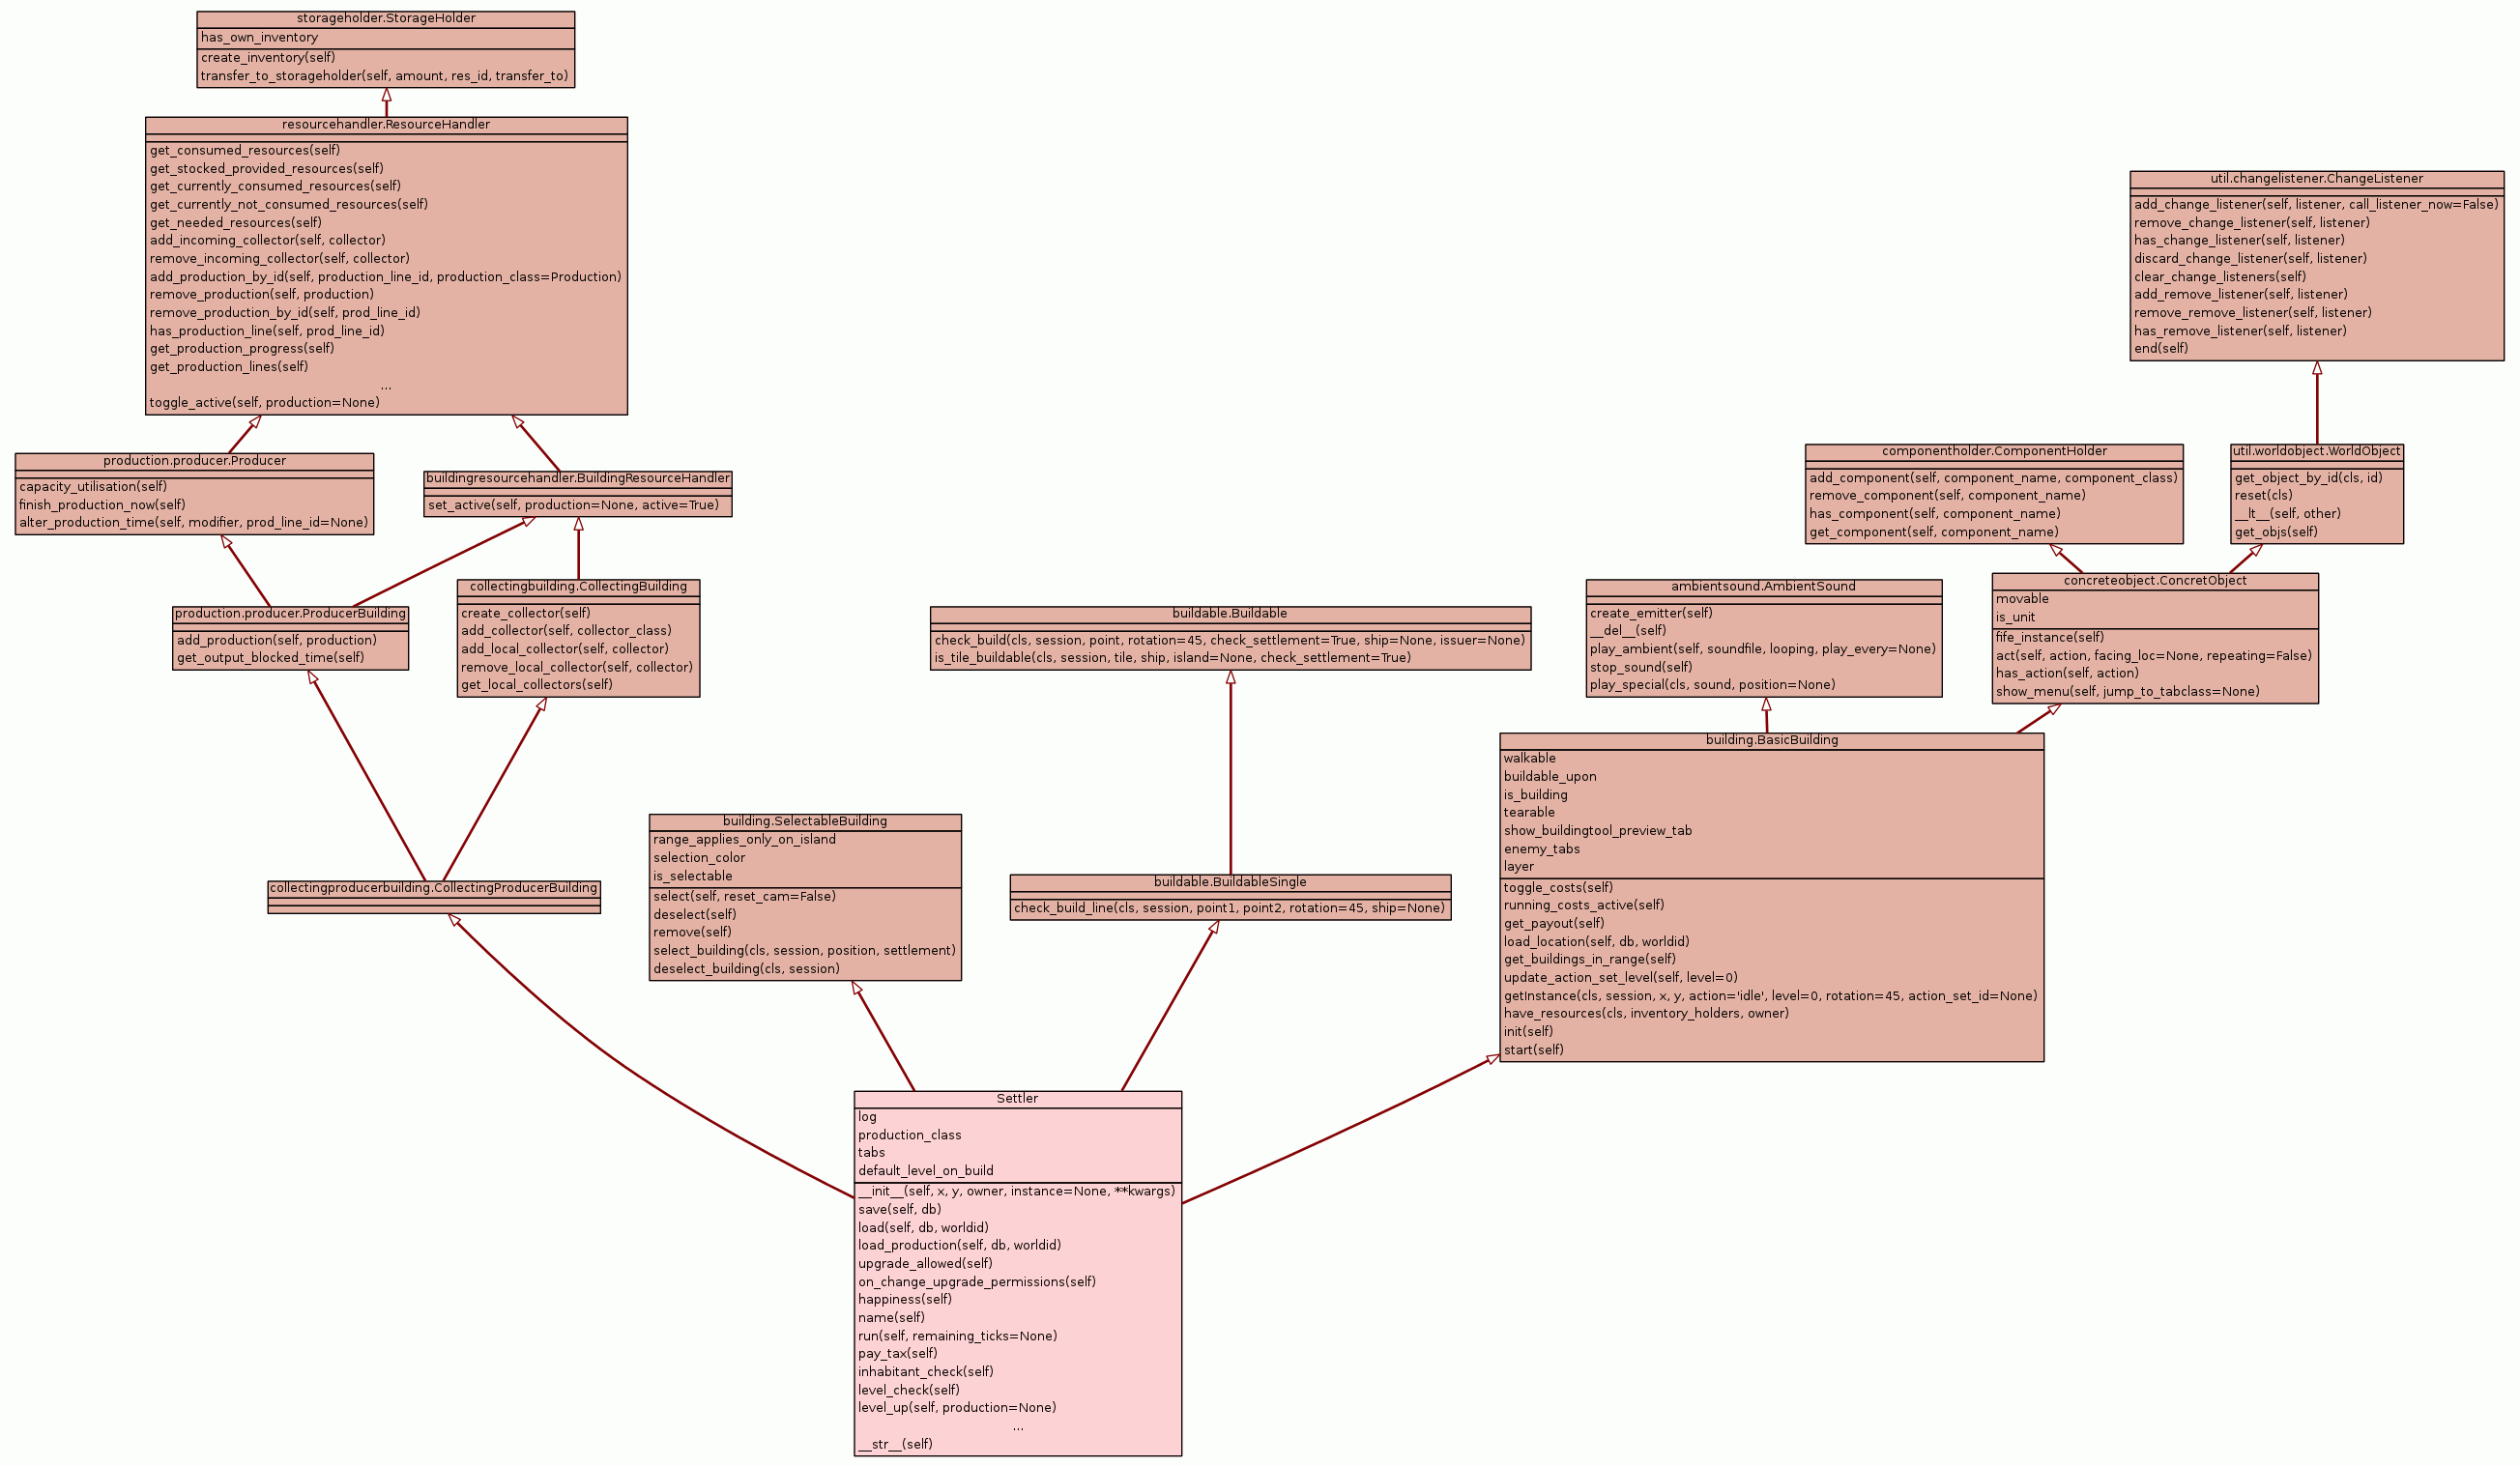
\includegraphics[angle=90,scale=0.25]{pics/settler_uml}
\caption{Inheritance tree for the \textit{Settler} class in \UH{}}
\label{fig:settleruml}
\end{figure}
The tree consists of 16 classes including many cases of multiple inheritance. 

Experience in working on this project has shown that making changes to any of the classes included in this tree is often
a very big task and comes with a great risk of introducing bugs into the code. It is also very difficult or even
impossible to write unit tests for these classes, as they are so dependent on each other and the game core, that it is
almost impossible to create the needed environment synthetically.

\paragraph{Settler Explained}
The \textit{Settler} class is comprised of 4 basic classes: \textit{BasicBuilding}, \textit{SelectableBuilding},
\textit{BuildableSingle} and \textit{CollectingProducerBuilding}. This is how most buildings in \UH{} are constructed. 

\textit{BasicBuilding} is a base class for every building, it loads graphics and provides
basic information like the name, position, owner and functionality for running costs and level upgrades.

\textit{SelectableBuilding} is a decorating class, that implements functions for selecting the building in-game. It
manages showing in-game menus and outlines. If a building is not supposed to be selectable, this class should not be
inherited.

\textit{BuildableSingle} is a decorating class which is used when building new buildings. It tells the game that it can
only be built as single instance, so there is no building of multiple instances at once. For this purpose the code
provides the \textit{BuildableLine}, \textit{BuildableRect}, etc. classes which can be used if needed.

\textit{CollectingProducerBuilding} is a collective class to make the Settler have collecting units which pick up
resources for usage and then produce something out of them. This is easier to demonstrate on a \textit{Lumberjack} for
example, he picks up trees and produces planks from it. The Settler consumes resources (food, textiles, etc.) and in
turn produces the abstract resource happiness.

\paragraph{Data-driven?}
\UH{} uses a SQLite\footnote{SQLite website: \url{http://www.sqlite.org/}} database to save parts of the object's
attributes. For example the size, health and name are saved in the database. This is necessary to make the higher level
classes in the architecture reusable for sub-classes. All buildings have a size, but it may be different from building
type to building type. It is saved to an external file to make it easily editable by non-programmers.

In summary I can say that the objects are partly data-driven, but usually it is not possible to add new buildings
without writing new code.

\subsubsection{RQ2}
In order to add a new building to \UH{} one has to look at the characteristics the building should have and
then find the appropriate classes from the \UH{} building classes collection. Those can then be combined to
form new buildings.

For example to create a settlement wall one could use the classes \textit{BuildableLine} and
\textit{BasicBuilding}. This is a very simple example which does not need to inherit many classes, as its functionality
is very limited. All attributes of this building can then be added in the database by using any SQLite database manager.

\subsubsection{RQ3}
Modifying existing in-game objects in \UH{} can be easy and very difficult. This depends on the degree of
change that is to be made. If only basic attributes like health, production time or similar are to be changed, then it
can easily be done by someone who knows his way around the database. If however new functionality is required, for
example a building which previously did not collect resources needs to collect resources, a change in the games code is
most certainly required. If the desired functionality exists, this can either be an easy task by just adding another class to
the hierarchy of the building or it can be very difficult if new functionality in the existing classes is required.

A good example for this is the boat builder, which is mainly a \textit{CollectingBuilding} producing units instead of
resources. The building has been implemented for over a year now and the team is still not certain if it works bug free
or not, as it required huge modifications to the production classes to be able to produce units instead of resources.

\subsubsection{RQ4}
There are no tools available to help with the addition/editing of content at this point. A map editor is being worked on
by two students of the \textit{Technische Universität München} in Germany. It will be available in future versions, but
it is not yet in a working state. Work is being done on the "\textit{editor}" branch of the official \UH{} git
repository\footnote{Link to the editor branch: \url{https://github.com/unknown-horizons/unknown-horizons/tree/editor}}.

\subsection{Battle for Wesnoth}
\BOW{} as described on the project's website:
\begin{quote}

\begin{center}
\includegraphics[scale=0.4]{pics/wesnothlogo}\end{center}

\textit{"The Battle for Wesnoth is a Free, turn-based tactical strategy game with a high fantasy theme, featuring both
single-player, and online/hotseat multiplayer combat. Fight a desperate battle to reclaim the throne of Wesnoth, or take
hand in any number of other adventures..."} -- from \url{http://www.wesnoth.org}
\end{quote}

\subsubsection{RQ1}
\BOW{} comes with its own markup language, \textit{WesnothMarkupLanguage} - \textit{WML}, to describe units, campaigns, AIs,
missions, maps, sounds, etc. \textit{WML} is similar to other markup languages like \textit{XML}, but more human readable and provides some basic functions to create logic - like basic if-clauses and variables. 

Entities are described in a component like way, but not all tags are components. For most tags like skills,
attacks and races components are used in code. Other attributes such as \textit{[portrait]} are not mapped to their own
component, but are just read as data for the basic unit class. 

\BOW{} parses all the tags in a config file into the config class where the single tags can be easily accessed by code.
The actual use of the tags is left to the code using the config. Classes like unit and race read values from the config
class.

To ease development it is also possible to access many internals using a LUA API. This is used for reading in
tags for maps and units. According to the development team the LUA API can be used for modding as well, this behavior
is not documented anywhere though \footnote{IRC logs regarding LUA API: \url{http://www.wesnoth.org/irclogs/2011/12/\%23wesnoth-dev.2011-12-08.log}}.

\paragraph{Data-driven?}
As all game content is described using \textit{WML}, \BOW{} can be seen as completely data-driven. Wesnoth contains an in-game option
to download other mods, containing new units, campaigns, etc. Within the concept of a round based strategy game the
engine is completely independent of the content.

\subsubsection{RQ2}
New objects are added to the game by adding a new file containing basic \textit{WML} with the description of the unit.
Since the game is fully moddable all units, maps and campaigns can be replaced just by editing and adding new files into
the basic directory structure \cite{wesnothaddunit}.

In order to add new \textit{WML} attributes, the c++ source-code has to be changed to recognize them. The \BOW{} parser
does not know anything about the tags it loads, therefore the only constraint is that the new tag should be used/accessed
in another c++ class, like the unit class, or LUA helper code.

\begin{lstlisting}[language=XML,caption=A basic (shortened) \BOW{} unit definition in WML, label=wesnothwml]
[unit_type]
    id=Elvish Lady
    name= _ "female^Elvish Lady"
    gender=female
    race=elf
    image="units/elves-wood/lady.png"
    profile="portraits/elves/lady.png"
    {MAGENTA_IS_THE_TEAM_COLOR}
    hitpoints=41
    movement_type=woodland
    movement=6
    experience=150
    level=3
    alignment=neutral
    advances_to=null
    {AMLA_DEFAULT}
    cost=10
    usage=null
    description= _ "Elves choose their leaders for their wisdom and sensitivity to the balance of universal forces; foresight is what has protected them in times of uncertainty. Their just reign is rewarded by the unflagging fealty of their people, which is the greatest gift for which any ruler could ask."
    [portrait]
        size=400
        side="right"
        mirror="true"
        image="portraits/elves/transparent/lady.png"
    [/portrait]
[/unit_type]
\end{lstlisting}

\subsubsection{RQ3}
To edit a unit in \BOW{} the \textit{WML} files have to be changed, nothing else has to be done. In order to change the
units behavior the c++ code has to be edited.

\subsubsection{RQ4}
\BOW{} comes with a set of tools to help developers and content creators. Wesnoth comes with a  map editor, tools to
validate user created \textit{WML} and provides an \textit{Eclipse}\footnote{Eclipse Project Homepage:
\url{http://www.eclipse.org}} plug-in, called \textit{"The Battle for Wesnoth UMC Development IDE"}\footnote{UMC Plugin
Website: \url{http://eclipse.wesnoth.org/}}.

It can setup
campaigns, races and more for the user, provides syntax highlighting for the WML and also some means of auto-completion. 
It can also launch the map editor and game with the specified campaigns and maps the user is working on and provides
means of using the WML validation tools. A screenshot of the WML editor is provided in \figref{fig:wesnothumc}.

\begin{figure}[H]
    \centering
    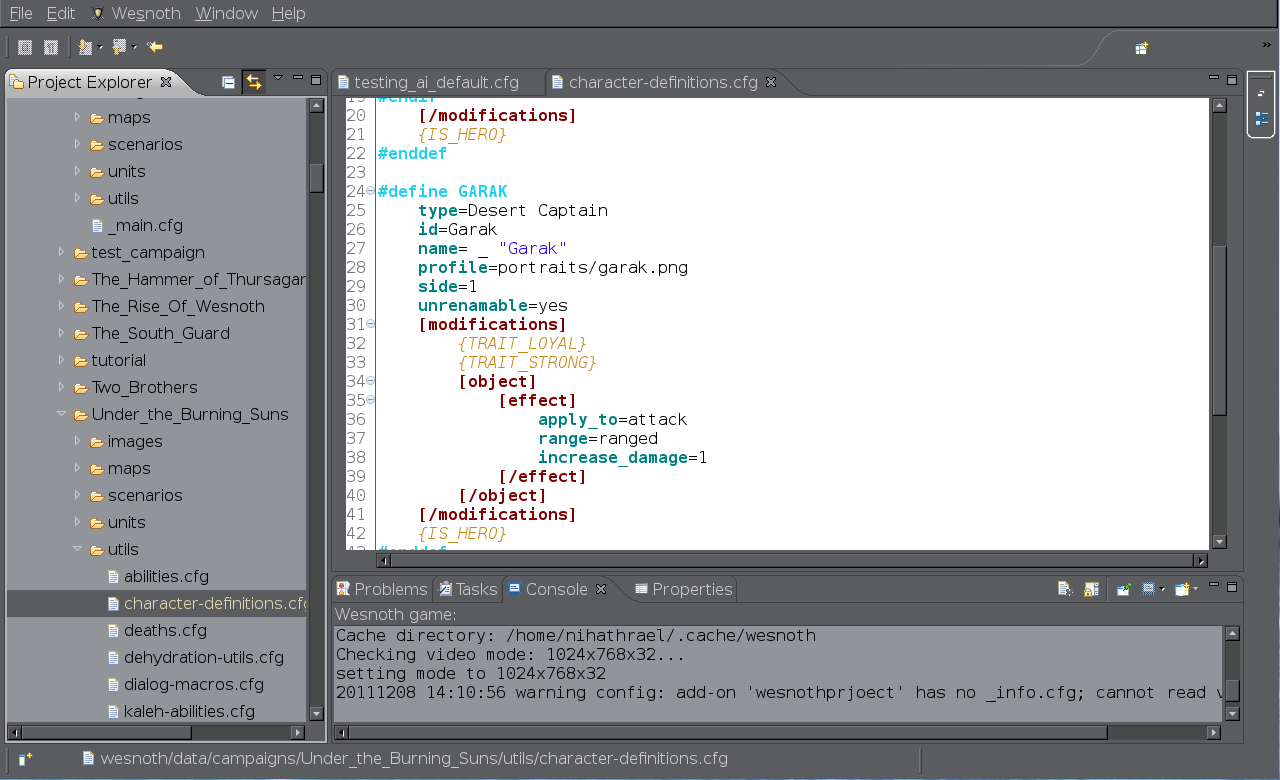
\includegraphics[width=\textwidth]{pics/wesnothumc}
    \caption{Wesnoth UMC Plugin WML editor}
    \label{fig:wesnothumc}
\end{figure}


\subsection{Mega Glest}
\GLEST{} as described on the project's website:
\begin{quote}

\begin{center}
\includegraphics[scale=0.5]{pics/glestlogo}\end{center}

\textit{"MegaGlest is a free and open source 3D real-time strategy (RTS) game, where you control the armies of one of
seven different factions: Tech, Magic, Egyptians, Indians, Norsemen, Persian or Romans. The game is setup in one of 16
naturally looking settings, which -like the unit models- are crafted with great appreciation for detail. Additional game
data can be downloaded from within the game at no cost."} -- from \url{http://www.megaglest.org}
\end{quote}

\subsubsection{RQ1}
\GLEST{} uses a mixture of inheritance and component-based object description. Basic things are set using
inheritance, for example the \textit{UnitType} class inherits from the \textit{ProducibleType} class, as every unit in
the game is producible. More advanced things are added to the unit as components, for example the \textit{UnitType} has
\textit{Level},\textit{SkillType}, \textit{Resource}, \textit{CommandType} and \textit{UnitParticleSystemType}
components. Units themselves are part of a bigger component hierarchy: Units are part of a \textit{FactionType}, which
is part of a \textit{TechTree}. See \figref{fig:glestclassh} for a detailed structure analysis. A class ending in
\textit{*Type} is used to represent prototypes for the actual instance classes. For example the \textit{UnitType} class loads all
necessary data from the XML definitions. In-game a \textit{Unit} instance is used, which itself contains a
\textit{UnitType} as information base.

\begin{figure}[h!]
    \centering
    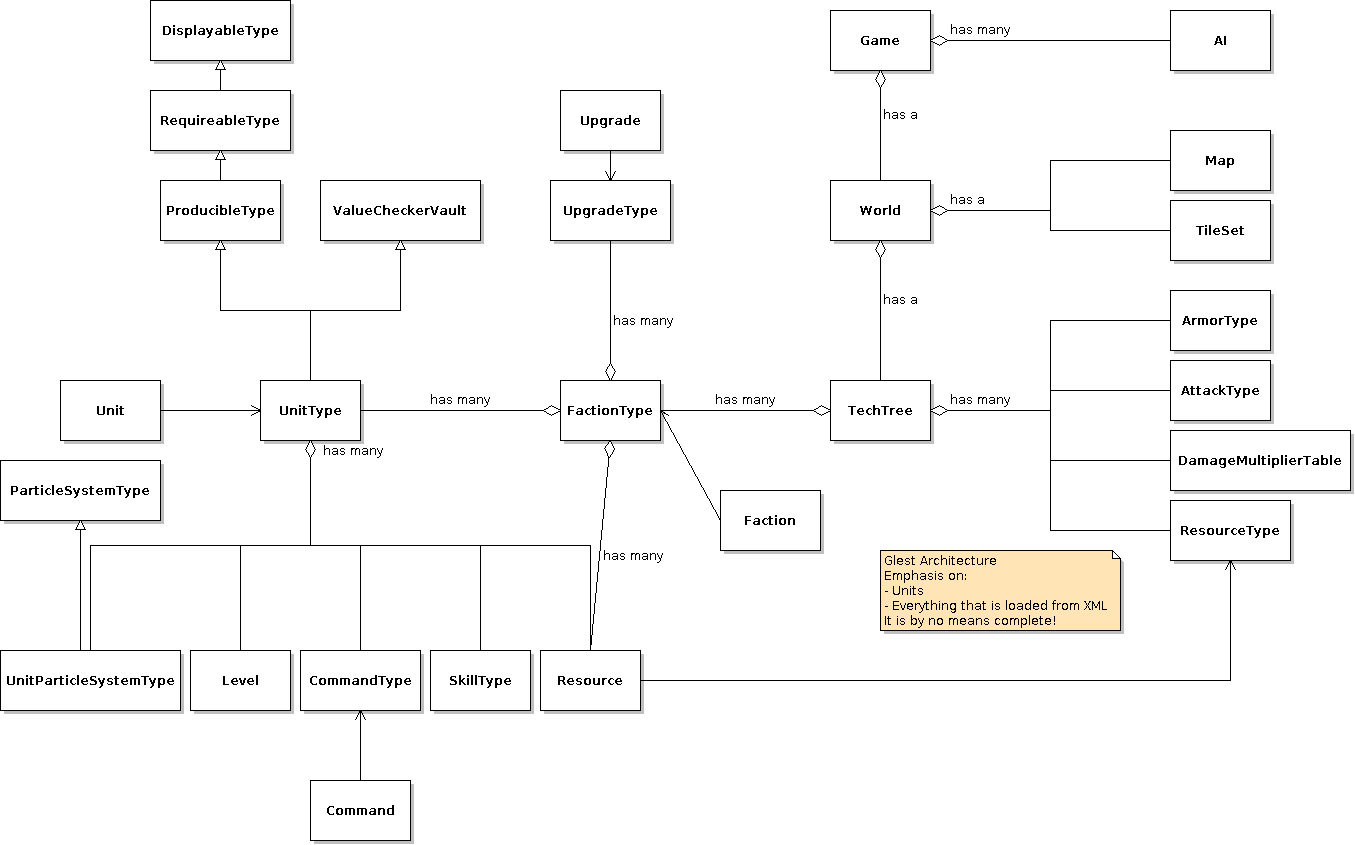
\includegraphics[angle=90,width=\textwidth]{pics/gamehierarchy}
    \caption{MegaGlest class hierarchy diagram}
    \label{fig:glestclassh}
\end{figure}

\paragraph{Data-driven?}
\GLEST{} is fully data-driven. All information needed for in-game objects, scenarios and campaigns is stored in XML files.
This makes \GLEST{} more of a game engine with a focus on real-time strategy than only a game. Several\footnote{List of
some mods: \url{http://www.moddb.com/games/megaglest/mods}} mods exist, proving that it is indeed possible to create new
games using \GLEST{} as a game engine. 

\subsection{RQ2}
In order to add new objects to \GLEST{}, new XML files have to be created. It can contain the definition of a unit, campaign,
tech tree or similar. See \listref{glestxml} for a shortened example of a basic unit definition. Every class has many
parameters which allow the user to specify the details for every unit. 

\begin{lstlisting}[language=XML,caption=A basic \GLEST{} (shortened) unit definition in XML, label=glestxml]
<unit>
	<parameters>
		<size value="1"/>
		<height value="2"/>
		<max-hp value="450" regeneration="5"/>
		<max-ep value="3000" regeneration="30"/>
		<armor value="15"/>	
		<armor-type value="leather"/>
		<sight value="12"/>
		<time value="200"/>	
		<multi-selection value="true"/>	
		<cellmap value="false"/>
		<levels>
			<level name="expert" kills="5"/>
			<level name="master" kills="15"/>
			<level name="legendary" kills="30"/>
		</levels>
</unit>
\end{lstlisting}

\subsubsection{RQ3}
In \GLEST{} editing objects is easy: Simply change the XML files to match the new requirements. Changing things in the
source code seems nicely doable as there are not too many inheritance based objects, instead composition is preferred.

\subsubsection{RQ4}
\GLEST{} comes with a map editor(\figref{fig:glestmapeditor}) to help with creating new maps to use in-game. It allows editing every possible detail
of the map and is thus of great help for content creators. 
\begin{figure}[H]
    \centering
    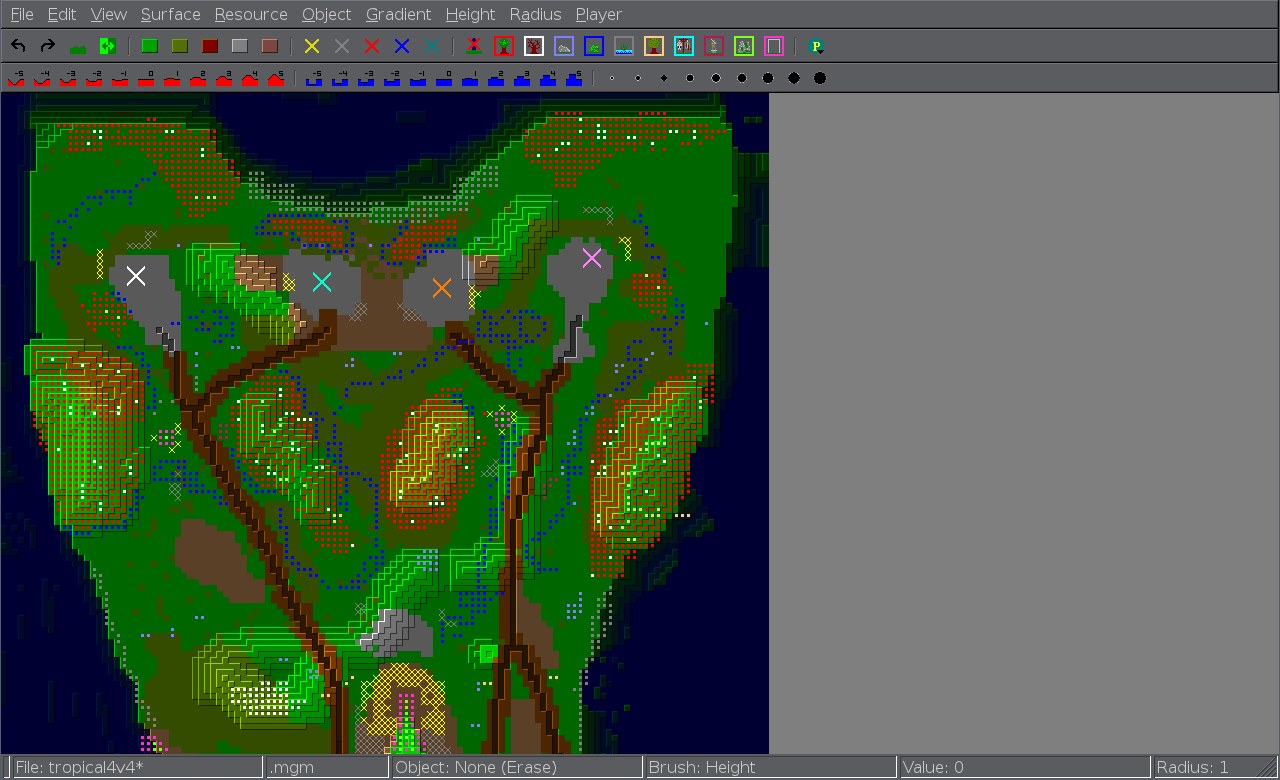
\includegraphics[width=0.75\textwidth]{pics/glesteditor}
    \caption{\GLEST{} map editor}
    \label{fig:glestmapeditor}
\end{figure}

\GLEST{} also comes with a model viewer, with which the
custom \textit{g3d} 3D model file format can be opened. It allows to view basic models and particle effects.

\begin{figure}[H]
    \centering
    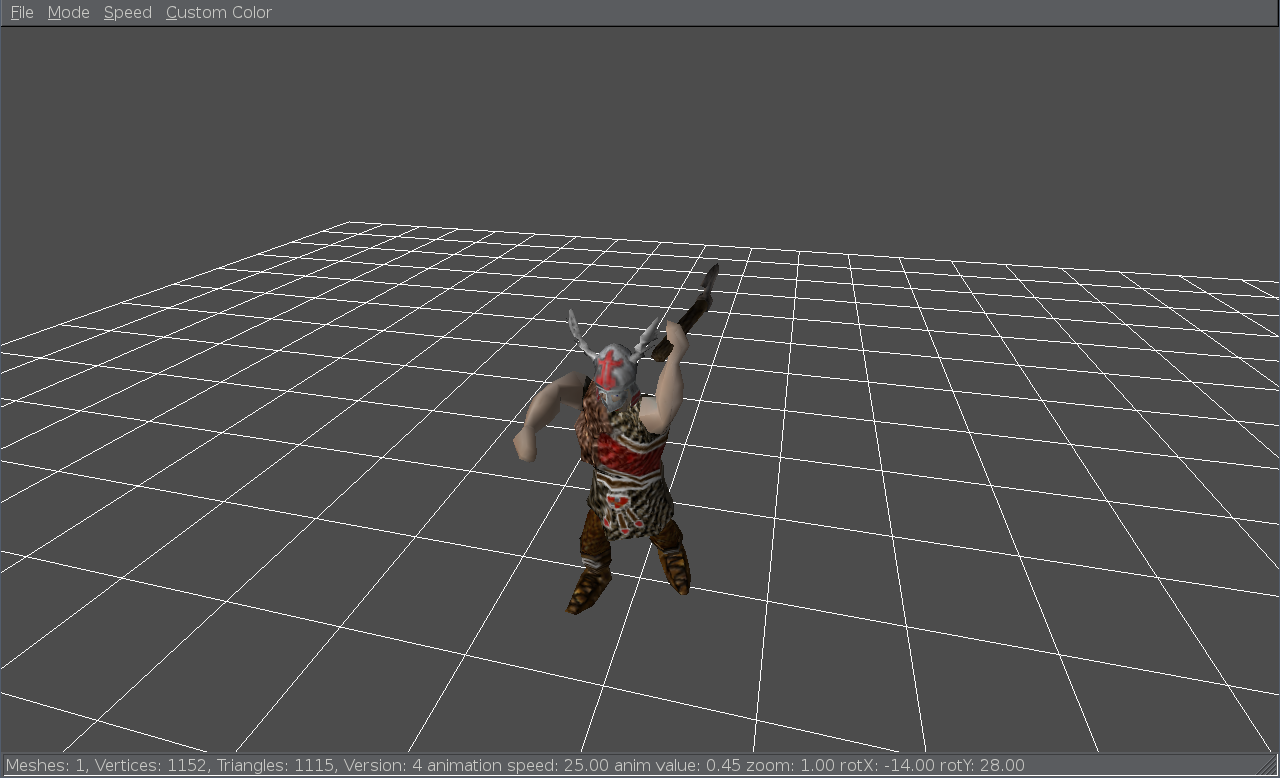
\includegraphics[width=0.75\textwidth]{pics/glestmodelviewer}
    \caption{\GLEST{} model and particle viewer}
    \label{fig:glestmodelviewer}
\end{figure}

\subsection{0 A.D.}

\AD{} as described on the project's website:
\begin{quote}
\begin{center}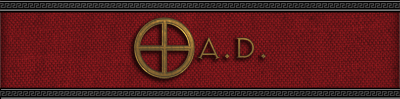
\includegraphics[scale=0.8]{pics/0ad}\end{center}
\textit{"0 A.D. (pronounced “zero ey-dee”) is a free, open-source, cross-platform real-time strategy (RTS) game of
ancient warfare. In short, it is a historically-based war/economy game that allows players to relive or rewrite the
history of Western civilizations, focusing on the years between 500 B.C. and 500 A.D. The project is highly ambitious,
involving state-of-the-art 3D graphics, detailed artwork, sound, and a flexible and powerful custom-built game engine."}
-- from \url{http://wildfiregames.com/0ad/}
\end{quote}

\subsection{RQ1}
\AD{} uses a completely component based approach to describe entities in the game. Units are described using a simple
XML based format, making up single units of many components. The engine provides components like \textit{Attack},
\textit{Cost}, \textit{Position} or \textit{VisualActor}. See \citet[Entity Component Documenation]{0adcomponents} for a
complete list and details. 

It is possible to implement components in c++ and JavaScript. The general idea is to use
JavaScript where possible and only use c++ if necessary for performance or communication with the game engine, for
instance for rendering. The components communicate with each other using a message based system or calling methods on
other components directly. The first approach is to be preferred, as the implementations remain separated from each other
this way. A component can send messages directly to a specific component type, or broadcast it to everything listening to
the specific message. A entity in the game is basically a number associated with a set of components. There is no
inheritance involved in creating an entity, other than inside a single component.

The engine allows to \textit{hot-load} components implemented in JavaScript, meaning changes in the JavaScript files will
be detected while the game is running and loaded into the engine. This enables the developer to make changes to the
components behavior while the game is running and directly seeing his results in-game.

\paragraph{Data-driven?}
\AD{} is completely data-driven. All information needed to construct a unit is saved in the basic XML format.
The XML format is specified by the components directly, making it easy to extend the markup language by new components.
As the game logic is implemented using these external components, it is easy to exchange the complete gameplay logic,
thus enabling very wide modding support and separating the game-play logic from the main engine.

\subsection{RQ2}
New objects can easily be added to the game by adding new XML unit entity definitions. No extra source-code is
necessary. A shortened sample unit definition is given in \listref{0adxml}.

\begin{lstlisting}[language=XML,caption=A basic \AD{} (shortened) unit definition in XML, label=0adxml]
<Entity parent="units/cart_cavalry_spearman_b">
  <Attack>
    <Melee>
      <Hack>6.0</Hack>
      <Pierce>16.0</Pierce>
    </Melee>
    <Charge>
      <Hack>18.0</Hack>
      <Pierce>48.0</Pierce>
    </Charge>
  </Attack>
  <Health>
    <Max>140</Max>
  </Health>
  <VisualActor>
    <Actor>units/carthaginians/cavalry_spearman_a.xml</Actor>
  </VisualActor>
</Entity>
\end{lstlisting}

\subsection{RQ3}
All units are defined using basic XML based definitions, making it easy to edit them with a normal text editor. No
changes to the code are necessary to edit any unit.

\subsection{RQ4}
\AD{} comes with an editor called \textit{Atlas}. It is a map and scenario editor and is not meant for editing unit
definitions. The editor is very similar to \GLEST{}'s editor in terms of features. It allows the user to edit any detail
of a map and comes with a unit viewer, that previews animations. A detailed user-manual is provided on the project's developer
pages \cite{0adeditor}.

Tool support for editing unit entity descriptions is not provided.

\subsection{Evaluation}
All four games provide data-driven approaches in varying degree.

\UH{} provides an SQLite driven approach, which usually requires editing some code to add new entities to the game. The
code is made up of huge inheritance trees, making it difficult to change the code or add new features. Storing the data
in an SQLite database makes it more difficult for contributors to change values, as they first have to learn how to use
an SQLite browser and understand how databases work. The plus side for this is, that relational queries are very fast.

\BOW{} and \GLEST{} allow the addition of units using basic markup languages like \textit{WML} and \textit{XML}. \BOW{}
provides basic means for scripting events and behavior using the \textit{WML} and possibly the LUA extension. Both
games use basic classes to which the data stored in the entity files is mapped, changing fundamental things about the
way the game behaves requires work on the code. Both games have separated the concerns by using a component similar
approach, making editing the source code easier than in \UH{}.

\AD{} is the only game in this study that uses a purely component based system. An entity in the game is represented by
a set of components tied to an ID, there are no base classes for units or buildings. They are entirely made up of
components. The engine allows scripting the components in JavaScript to ease development, but provides the possibility to
easily port components to c++, should speed be a problem. Components written in JavaScript can be hot-loaded during the run-time
of the game, making it easy to debug and work on single parts of the game and directly seeing the impact on the game.
The implementation of \AD{} is very similar to the system described in \cite{Fh02ageneric}, but it does not use the
enhanced component in and output system. Instead it uses the QT like described version of messages between components.

\section{Transferring the Results to \UH{}}
Looking at the ease of content creation of \BOW{}, \GLEST{} and \AD{} it becomes clear that \UH{} is not nearly as
flexible and easy to use as the other projects. While \AD{} has the cleanest component based architecture, it is not
possible to transfer the design completely to \UH{}. 

As the current code is not a component driven design, it is very difficult to convert the entire code structure to a
component based architecture in one big refactoring. Therefore a middle ground has to be found here, where the code can
be refactored and changed to components in small parts. The difference between c++ and JavaScript components is not suitable
for \UH{} as it is written entirely in Python, so there is no possibility to differentiate between compiled and scripted
components.

An implementation similar to \BOW{} or \GLEST{} seems useful, keeping in mind the specific requirements for \UH{}.

